\section{System development I: Image pre-processing}

Described in this section are the approaches considered for noise removal, image segmentation and binary image pre-processing, most of which were pre-existing within ImageJ. As one of the initial aims in designing the system was minimisation of execution time, speed of execution was prioritised when selecting a method for each pre-processing stage.

\subsection{Low-frequency noise removal}

The first stage in any image processing algorithm generally involves an attempt to minimise any unwanted noise or distortion present in a given image. Low-frequency noise is typically characterised by a gradient across the image plane, resulting from, for example, non-uniform illumination. Removing this gradient results in a more homogeneous background, which is preferable for image segmentation (see below), and may be accomplished in a variety of ways.

\subsubsection{Mean filtering and background subtraction}

A mean filter is a form of smoothing filter that can be used to suppress high-frequencies in an image. A simple example of a mean filter kernel is as follows:

\begin{equation}
	G_{n,n} = \frac{1}{n^2}
	 \begin{bmatrix}
	  1 & 1 & \cdots & 1 \\
	  1 & 1 & \cdots & 1 \\
	  \vdots  & \vdots  & \ddots & \vdots  \\
	  1 & 1 & \cdots & 1 
	 \end{bmatrix}
\end{equation}

\noindent where $G_{n,n}$ is a square matrix and $(n-1)/2$ is the filter radius. If $G$ is convolved with an image ($I$), each pixel in the output image ($J$) is therefore defined as:

\begin{equation}
	J(x,y) = \frac{1}{n^2}\sum^{m}_{j=-m}\sum^m_{i=-m}I(x+i,y+j)
\end{equation}

\noindent where $2m=n-1$. By forming a duplicate of the image to be filtered and smoothing over a sufficiently large radius, all details (high frequencies) in the image are suppressed and an approximation of the image background results. This \lq background image' may then be subtracted from the original, leaving the object(s) of interest intact against a uniform background. However, convolution with a smoothing filter with a large kernel is computationally expensive, with the processing time being proportional to $n^2 \times \mbox{image area}$.

\subsubsection{Frequency-domain filtering}

Noise removal may also be effected by filtering in the frequency domain rather than using spatial filtering. The Fourier transform of an image is computed, the result convolved with the desired filter and the inverse-Fourier transform calculated, resulting in the original image with noise removed. However, this approach is also very time-consuming, particularly for large images.

\subsubsection{Rolling ball background subtraction}

This approach to background removal may be conceptualised as follows. If the image to be filtered is considered to be three-dimensional, the third dimension being the luminous intensity at each pixel, the image will resemble a surface with depressions (Fig.~\ref{fig:PelletSurfacePlot}). If the filter kernel is considered to be a ball of radius $r$ that traverses this surface, the background is defined as any part of the surface that contacts the ball. The objects within the image, represented by \lq holes' in the surface plot, will be unaffected if $r$ is sufficiently large. The ImageJ implementation is based on Sternberg's rolling ball algorithm \cite{sternberg1983} and, as it is far less time-consuming than smoothing or frequency-domain filtering, was selected as the preferred means of background removal.

\begin{figure}[tb]
	\centering
	\subfloat{\fbox{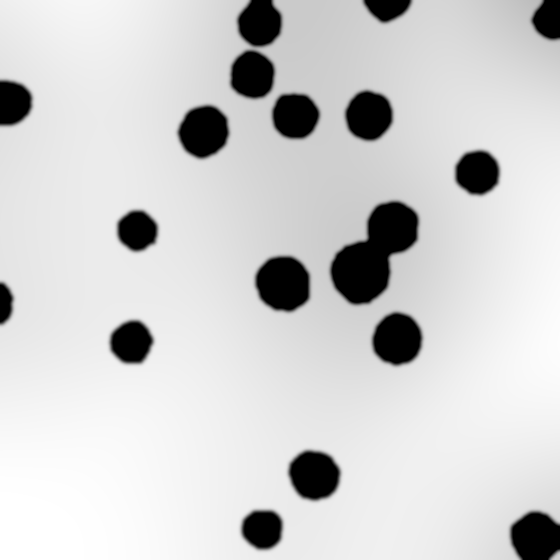
\includegraphics[width=5cm]{../C2/PelletPlot}}}
	\hspace{1.5cm}
	\subfloat{\fbox{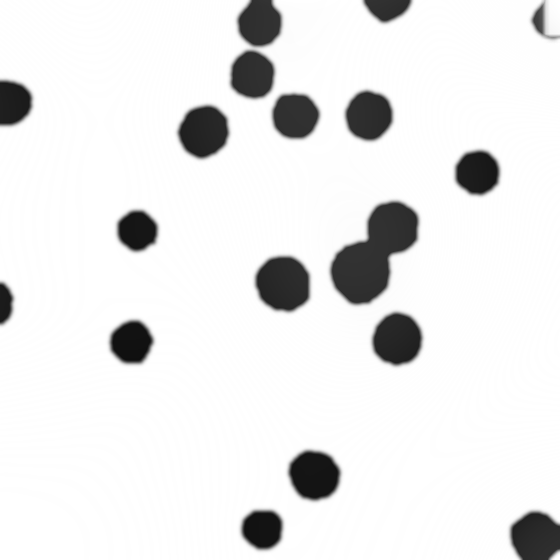
\includegraphics[width=5cm]{../C2/PelletPlotII}}}
	\\
	\subfloat{\pstool[width=6cm]{../C2/PelletSurfacePlot}{
		\psfrag{x}[Bc]{\al $x$}
		\psfrag{y}[Bc]{\al $y$}
		\psfrag{255}[Bc]{\al 255}}
	}
	\hspace{0.5cm}
	\subfloat{\pstool[width=6cm]{../C2/PelletSurfacePlotII}{
		\psfrag{x}[Bc]{\al $x$}
		\psfrag{y}[Bc]{\al $y$}
		\psfrag{255}[Bc]{\al 255}}
	}
  \caption{Surface plots of an image, before (left) and after (right) background subtraction, showing objects as depressions in the surface.}
  \label{fig:PelletSurfacePlot}\end{figure}

\subsection{High-frequency noise removal}

High-frequency \lq speckle' noise can result from, for example, electrical noise in the CCD array on which the image was captured and is characterised by individual pixels within an image that are noticeably different in intensity from their immediate neighbours, resulting in a \lq granular' appearance (Fig.~\ref{fig:Noise}). A common approach to alleviating this problem is median filtering, a form of \lq rank filtering', so called because the pixel values within a specified radius are \lq ranked' according to their intensity values and the median selected as the filter output. This is a more effective form of high-frequency noise removal than smoothing, as fine details such as edges and region boundaries are preserved (Fig.~\ref{fig:HighFreqNoise}). Median filtering was therefore chosen as the means of high-frequency noise removal for this study.

\begin{figure}[t]
	\centering
	\subfloat[]{\label{fig:Noise}\fbox{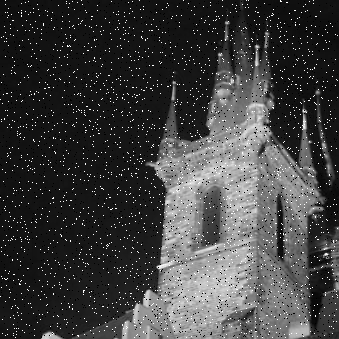
\includegraphics[width=5cm]{../C2/Noise}}}
	\hspace{1cm}
	\subfloat[]{\fbox{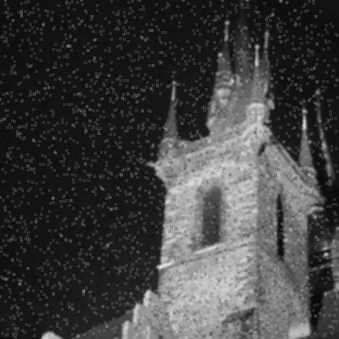
\includegraphics[width=5cm]{../C2/Mean}}}
	\\
	\subfloat[]{\fbox{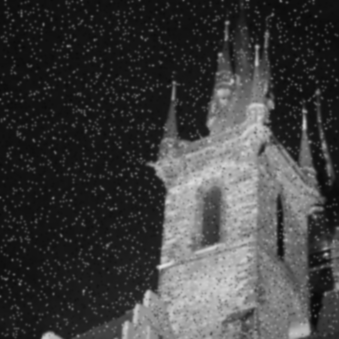
\includegraphics[width=5cm]{../C2/Gauss}}}
	\hspace{1cm}
	\subfloat[]{\fbox{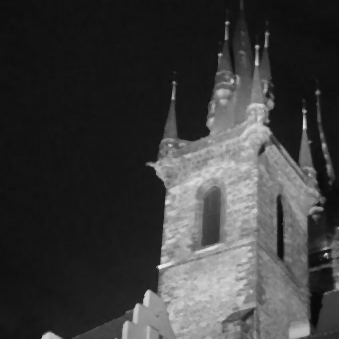
\includegraphics[width=5cm]{../C2/Median}}}
  \caption{(a) Image in Figure~\ref{fig:Digitise} with added \lq{}salt and pepper' noise (b) Result of mean filtering (c) Result of Gaussian filtering (d) Result of median filtering. In all cases, the filter radius was 1 pixel.}
  \label{fig:HighFreqNoise}
\end{figure}

\subsection{Image segmentation}

Image segmentation, in the simplest sense, refers to the separation of objects of interest from the background. This is achieved by specifying regions within the image, based on a particular property, with each region being relatively homogeneous with respect to the chosen property and differing from the other regions of the image. One of the simplest means of implementing image segmentation is grey-level thresholding, which defines different regions within an image based on the grey level of individual pixels. A binary image, $g(x,y)$, may be generated from a grey-level image, $f(x,y)$, as follows:

\begin{equation}
	g(x,y) = \left\{ \begin{array}{l l l}	1 & \mbox{ for } & f(x,y) \geq T \\
																						0 & \mbox{ for } & f(x,y) < T \end{array} \right.
\end{equation}

\noindent where $T$ is some pre-determined \lq threshold' that results in optimal separation between object and background. A value of $T$ may be calculated for the entire image (a global threshold) or $T$ may vary between different areas of the image, being dependent on image properties within a specified window (local or \lq adaptive' thresholding \cite{wilkinson1998}). The calculation of a value for $T$ based on the image histogram (i.e., the grey-level distribution of the image) is a common approach \cite{wilkinson1998}. If both the object of interest and the image background have relatively homogeneous grey levels (and no other regions are present in the image), then the image histogram should be approximately bi-modal (Fig.~\ref{fig:BiModalHist}). In this scenario, the calculation of a threshold is intuitive and will lie approximately at the location of the local minimum between the two modes.

\begin{figure}[t]
	\centering
	\setlength{\unitlength}{1cm}
	\begin{picture}(10,7.5)
		\put(1.2,1){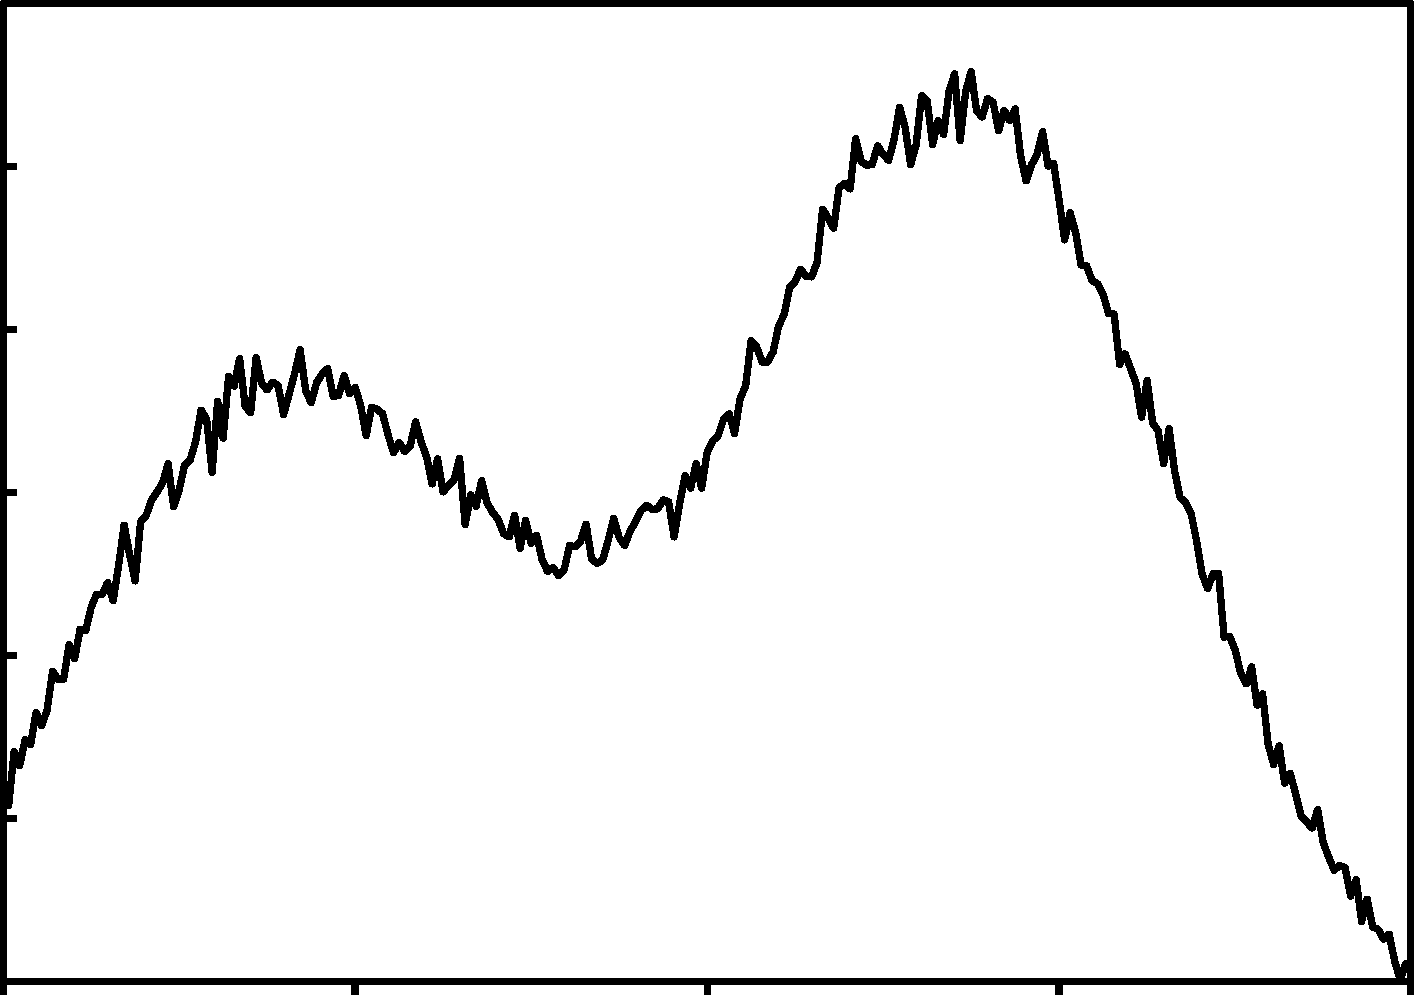
\includegraphics[width=8.5cm]{../C2/BiModalHistogram}}
		\put(4.5,0){Grey Level}
		\put(1.1,0.5){0}
		\put(3.1,0.5){64}
		\put(5.1,0.5){128}
		\put(7.2,0.5){192}
		\put(9.4,0.5){256}
		\put(0,3){\rotatebox{90}{Frequency}}
		\put(0.6,1.0){0.0}
		\put(0.6,1.95){0.1}
		\put(0.6,2.9){0.2}
		\put(0.6,3.9){0.3}
		\put(0.6,4.9){0.4}
		\put(0.6,5.85){0.5}
	\end{picture}
	\caption{A bi-modal image histogram, representing two distinct regions within the image with differing grey-level distributions.}
	\label{fig:BiModalHist}
\end{figure}
	
Real images rarely exhibit such ideal characteristics and as a result, the calculation of a threshold is non-trivial in many cases. Often there may be no discernible peaks or valleys in the image histogram or there may be considerable overlap between modes representing object and background. The choice of algorithm for threshold computation therefore depends very much on the nature of the image and the shape of the histogram. For example, the \lq triangle' thresholding technique \cite{zack1977} is quite effective for histograms in which the background mode is significantly larger than that of the object, characteristic of a large image containing small, low-contrast objects. However, this approach requires \lq smoothing' of the image histogram for accurate segmentation, necessitating the estimation of further variables (the width of the smoothing kernel and the number of smoothing iterations), and is biased toward computing relatively high threshold values (Fig.~\ref{fig:MyceliaTriangleThresh}).

Another useful technique is that proposed by Otsu, which seeks to maximise the inter-regional variance ($\sigma^2$) in the segmented image \cite{wilkinson1998}:

\begin{equation}
	\sigma^2 (T) = \frac{[\overline{I}_t P(T) - \overline{I}(T)]^2}{P(T)[1-P(T)]}
\end{equation}

\noindent where $\overline{I}_t$ is the mean grey value of the entire image, $P(T)$ is the probability of a pixel having a grey level $\leq T$ and $\overline{I}(T)$ is the mean grey level of those pixels. The optimum threshold is determined as that which maximises $\sigma^2 (T)$. While this approach yielded acceptable results in the case of mycelial images (Fig.~\ref{fig:MyceliaOtsuBin}), the computational overhead is relatively large.

The iso-data algorithm \cite{ridler1978}, the default thresholding method in ImageJ, determines a threshold by selecting an initial value (such as the minimum grey level in an image) and then calculating the mean values of all pixels above this value (the \lq background' pixels) and all pixels below (the \lq object' pixels). The value of $T$ is increased until the following condition is met:

\begin{equation}
	T \geq \frac{\mbox{object mean} + \mbox{background mean}}{2}
\end{equation}

\noindent This method of thresholding proved effective provided that the hyphae were contiguously stained a uniform colour and they were presented against a homogeneous background (Fig.~\ref{fig:MyceliaIsoThresh}).

\begin{figure}[tb]
	\centering
	\subfloat[]{\label{fig:MyceliaPreThresh}\fbox{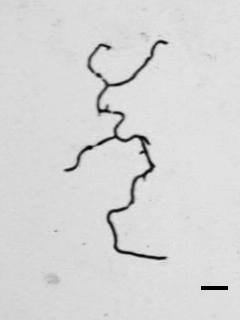
\includegraphics[width=3.1cm]{../C2/MyceliaProca}}}
	\hspace{0.2cm}
	\subfloat[]{\label{fig:MyceliaTriangleThresh}\fbox{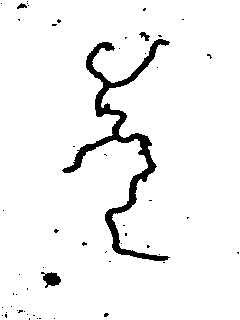
\includegraphics[width=3.1cm]{../C2/MyceliaTriangleBin}}}
	\hspace{0.2cm}
	\subfloat[]{\label{fig:MyceliaOtsuBin}\fbox{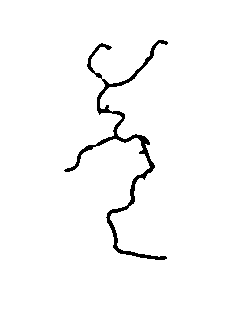
\includegraphics[width=3.1cm]{../C2/MyceliaOtsuBin}}}
	\hspace{0.2cm}
	\subfloat[]{\label{fig:MyceliaIsoThresh}\fbox{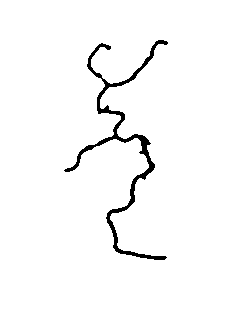
\includegraphics[width=3.1cm]{../C2/MyceliaProcc}}}
  \caption{(a) Original image of stained mycelium (Bar 30~$\mu$m) with binary images resulting from application of (b) triangle-thresholding (c) Otsu thresholding and (d) iso-data thresholding.}
  \label{fig:MyceliaThresh}
\end{figure}

\subsection{Pre-processing of binary images}\label{sec:BinPreProc}

\subsubsection{Morphological filtering}

Once thresholding is complete and a binary image has been generated, a degree of enhancement is required using morphological filters prior to object classification and subsequent measurement. For example, such processing may be necessary to remove small, unwanted objects (artifacts) or fill small holes or gaps within objects of interest. Small artifacts may be removed from an image by one or more \emph{erosion} operations, while the quasi-inverse is termed \emph{dilation}, both of which are illustrated in Figure~\ref{fig:BinMorph}. In simple terms, \emph{erosion} may be considered to \lq shrink' objects, while \emph{dilation} causes them to \lq grow'. More specifically, \emph{erosion} may be explained as follows. Let $H$ be a structural element consisting of some arrangement of foreground pixels. An image ($I$) is traversed by $H$ and each pixel $(i,j)$ in the output image ($J$) is defined as follows for every $(i,j) \in I$:

\begin{equation}
	J(i,j) = \begin{cases} 0 & \mbox{if } H_{i,j} \subseteq O\\
																			1 & \mbox{otherwise}
												\end{cases}
\end{equation}

\noindent where $O$ is a foreground object and $H_{i,j}$ represents $H$ centred on $(i,j)$.  Put simply, if $H$ is entirely contained within $O$ when centred at a position $(i,j)$, then $(i,j)$ is defined as foreground in the output image. Otherwise it is denoted as background. \emph{Dilation} is somewhat the reversal of \emph{erosion}:

\begin{figure}[tb]
	\centering
	\subfloat[]{
		\begin{tabular}{m{3.1cm} m{0.5cm} m{3.1cm} m{0.5cm} m{3.1cm}}
			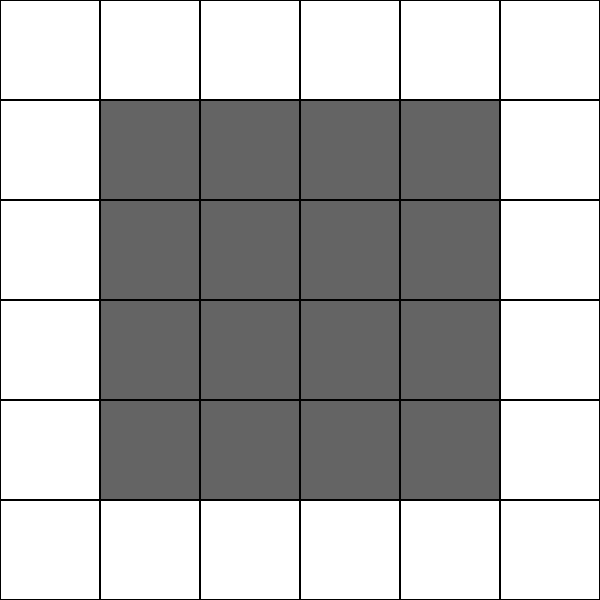
\includegraphics[width=3cm]{../C2/PixObject} &
			$\mathbf{\ominus}$ &
			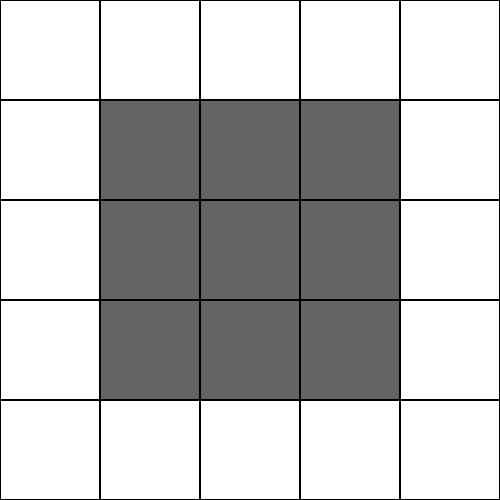
\includegraphics[width=2.5cm]{../C2/StructElement} &
			$\mathbf{=}$ &
			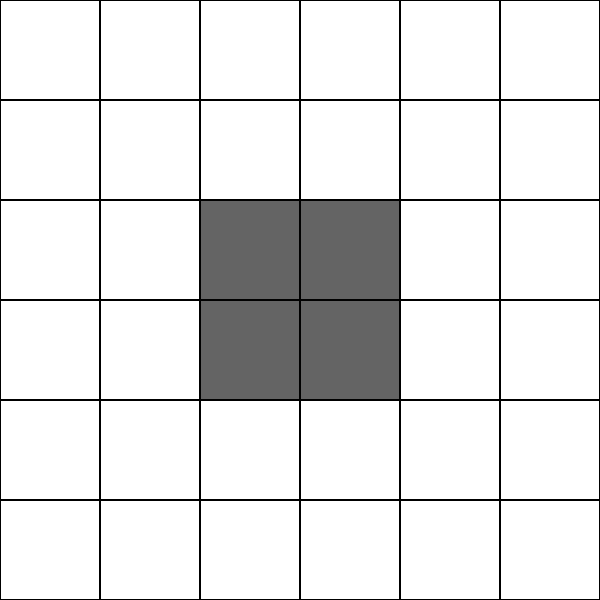
\includegraphics[width=3cm]{../C2/PixelErosion}
		\end{tabular}
	} \\
	\subfloat[]{
		\begin{tabular}{m{3.1cm} m{0.5cm} m{3.1cm} m{0.5cm} m{3.1cm}}
			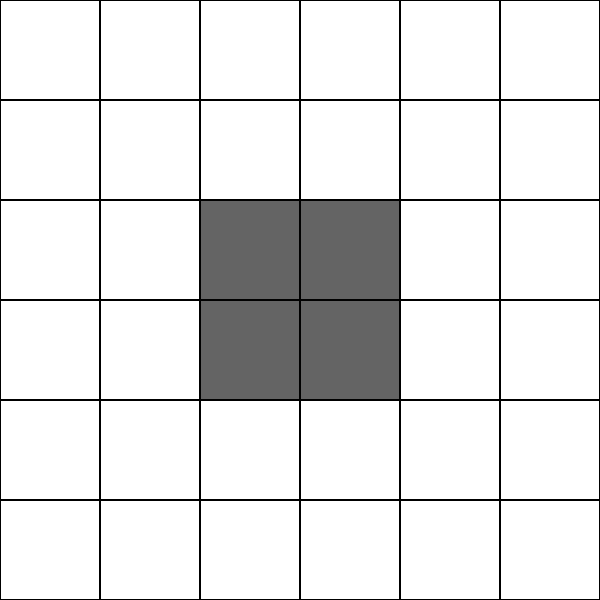
\includegraphics[width=3cm]{../C2/PixelErosion} &
			$\mathbf{\oplus}$ &
			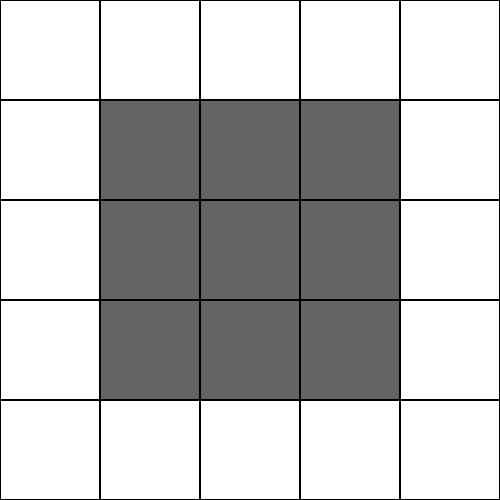
\includegraphics[width=2.5cm]{../C2/StructElement} &
			$\mathbf{=}$ &
			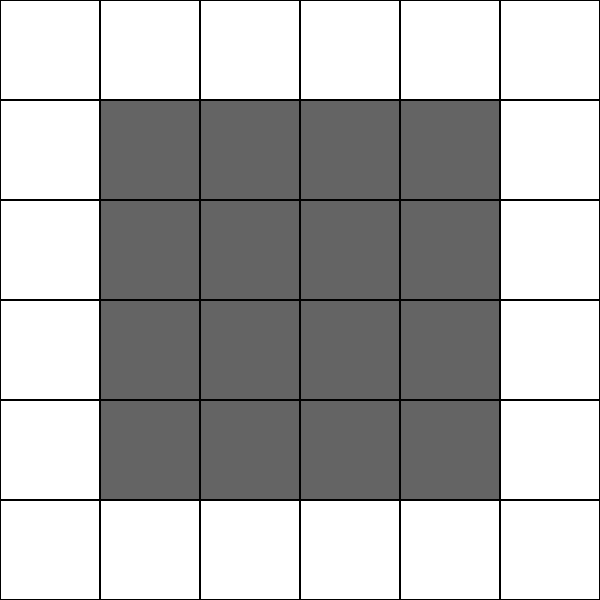
\includegraphics[width=3cm]{../C2/PixObject}
		\end{tabular}
	}
  \caption{Effect of (a) \emph{erosion} (denoted by $\ominus$) and (b) subsequent \emph{dilation} (denoted by $\oplus$) on a binary object. This combined sequence is commonly termed an \emph{open} operation.}
  \label{fig:BinMorph}
\end{figure}

\begin{equation}
	J(i,j) = \begin{cases} 0 & \mbox{if } (i,j) \in H_{m,n} \mbox{ for any } (m,n) \in O\\
																			1 & \mbox{otherwise}
												\end{cases}
\end{equation}

\noindent $H$ is centred on each foreground pixel in $O$ and any background pixels in $I$ overlapped by $H$ are designated as foreground pixels in $J$.

\subsubsection{Watershed segmentation}

It is often the case that objects within binary images are in contact with one another (Fig.~\ref{fig:TouchObjects}). In the case of binary images of relatively spherical structures (such as fungal spores or pellets), some form of \emph{watershed} segmentation may be employed to separate touching objects, which is based on the concept of constructing boundaries (\lq watersheds') between adjacent objects or regions. The ImageJ implementation is based on the generation of a Euclidean Distance Map (EDM) \cite{leymarie1992}, a visual representation of the distance between each foreground pixel and the nearest background pixel (Fig.~\ref{fig:DistanceMap}). Each foreground pixel is assigned an integer value (represented by different grey levels in the visual representation) corresponding to the number of pixels separating it from the nearest background pixel. Alternatively, this value could be considered the number of \emph{erosion} operations that would be required to remove this pixel from the image. From the EDM image, a further image is generated, displaying the \lq ultimate points', or the local maximum values for each EDM (Fig.~\ref{fig:UltimatePoints}). These \lq ultimate points' can be thought of as approximations to the centre of each object. It remains to reconstruct the original image by way of conditional \emph{dilation}; that is, a number of \emph{dilations} are performed on each object, sufficient to restore the object to its original size, on condition that \emph{dilation} causes no two objects to come into contact with each other (Fig.~\ref{fig:Watershed}). \emph{Watershed} segmentation has been utilised in other studies of fungal morphology \cite{ocleirigh2003,bizukojc2009} and was deployed in this study to separate touching objects in images of spores and pellets.

\begin{figure}[tb]
	\centering
	\subfloat[]{\label{fig:TouchObjects}\fbox{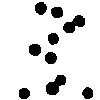
\includegraphics[width=4cm]{../C2/TouchObjects}}}
	\hspace{1cm}
	\subfloat[]{\label{fig:DistanceMap}\fbox{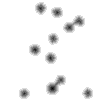
\includegraphics[width=4cm]{../C2/DistanceMap}}}
	\\
	\subfloat[]{\label{fig:UltimatePoints}\fbox{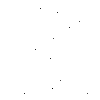
\includegraphics[width=4cm]{../C2/UltimatePoints}}}
	\hspace{1cm}
  \subfloat[]{\label{fig:Watershed}\fbox{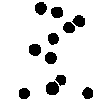
\includegraphics[width=4cm]{../C2/Watershed}}}
  \caption{(a) Original image containing conjoined objects (b) Euclidean Distance Map (c) Ultimate Points (d) Segmentation of objects following conditional \emph{dilation}.}
  \label{fig:WatershedSeg}
\end{figure}

\subsubsection{Object classification}

Prior to measurement, it is necessary to identify different objects within the image, such as spores, hyphae and any remaining unwanted artifacts. This may be achieved by assigning certain descriptors to each object, such as the projected area, perimeter length, equivalent diameter or some measure of boundary curvature, the most common form of which in the study of microbes is circularity. Other parameters, such as Fourier descriptors \cite{pazoti2005} and chain codes \cite{wilson2002}, may also be of value.

To maximise the accuracy of object classification, a training set can be utilised, the establishment of which requires each object in an image to be quantified in terms of $\Ap$ and $P$, for example, which subsequently form the elements of a feature vector for that object \cite{mangasarian1995}. The object is then classified as a spore, hypha, mycelium or artifact by a human observer and this process continues until a sufficiently large knowledge base has been established. When a test object is subsequently presented, a feature vector is formed and, for example, the Euclidean Distance calculated between the vector of the test object and those in the knowledge base. The test object is classified according to the \lq winning' vector in the knowledge base, that is, the vector within the knowledge base containing the features that best describe the test object. However, such an approach involves a large number of calculations and requires time devoted to the establishment and maintenance of the knowledge base. A similar approach involves the implementation of some form of Artificial Neural Net (ANN), such as that adopted by Papagianni and Mattey for the classification of fungal structures \cite{papagianni2006a}.

However, the most common (and least time-consuming) means of discriminating between objects of differing classes in the quantification of fungal morphology is the use of threshold values \cite{pinto2004,anikster2005}. In this study, minimum and/or maximum values were set for projected area ($\Apm$) and circularity ($\Csm$, $\Chm$) and these values were refined by analysing the distribution of $\Ap$ and $C$ within a population (see Section~\ref{sec:KinSporeSwell}). Establishment of values for these variables will be discussed in Section~\ref{sec:KinSporeSwell} and the effect of small variations in these values is investigated in Sections~\ref{sec:KinSporeSwell} and \ref{sec:KinHyphDev}.

\subsubsection{Pre-processing of hyphal structures}

Prior to the measurement of hyphal architecture, it is common for the associated binary images to be subjected to some form of thinning algorithm to produce a skeletal structure \cite{spohr1998,tucker1992,denser-pamboukian2002}. This facilitates the rapid determination of parameters such as the total length of the mycelium, the total number of tips and the location of branch-points. For relatively low-resolution images of mycelia, in which the hyphae are typically just a few pixels in diameter, \emph{skeletonisation} may be achieved quickly and accurately. However, such an approach may not be suitable for higher resolution images, resulting in large hyphal \lq objects' or regions, small changes in the shape of which can result in significantly different skeletal structures \cite{sonka1993}. ImageJ's implementation of a thinning algorithm is based on that of Zhang and Suen \cite{zhang1984}, in which pixels are iteratively removed, by way of a look-up table, until a skeleton remains. Some of the limitations of this approach will be addressed in the next section.